\section{Evaluation}

For testing strategy, we adhere to previous state-of-the-art models to ensure comparability.
The datasets used for the evaluation are Tanks and Temples~\cite{tankstemples}, MipNeRF360~\cite{mipnerf360}, LLFF~\cite{mildenhall2019llff} and DTU~\cite{dtu}.

\paragraph{Implementation Details.}
The Tanks and Temples dataset covers real-world indoor and outdoor scenes, but we only use a subset of 8 scenes, as done by other sparse-view models like \textit{Intern-GS} and \textit{InstantSplat}. We focus on the 3-view setting and therefore use the same train/test split. This means the testing set includes 12 images uniformly sampled without the first and last frame and the remaining set is the training set where we again uniformly sampled the 3 views~\cite{InstantSplat}. For Tanks and Temples, no downsampling is applied.

The MipNeRF360 dataset contains real-world $360^\circ$ indoor and outdoor scenes. For this dataset, two different approaches are used. One for the 3-view setting as defined by \textit{Gaussian Scenes}~\cite{GaussianScenes} and one for the 12-view setting as defined by \textit{SparseGS}~\cite{SparseGS}. For both settings, the 4x downsampled images are used, to adhere to the evaluation strategies of state-of-the-art models.  For the 3-view setting, we use every 8th image as testing set and uniformly sample the 3 training views. For the 12-view setting, we use the split dataset provided by \textit{SparseGS}~\cite{SparseGS}. The 12-view setting uses only 6 of the 9 scenes contained in the MipNeRF360 dataset, whereas the 3-view setting uses all 9 scenes.

The LLFF dataset contains real-world forward-facing images. For this dataset, we used the same evaluation strategy as defined by \textit{DNGaussian}. A downsampling rate of 8 is used, and we adhere to the train/test split of the 3-view setting of \textit{DNGaussian}~\cite{DNGaussian}.

Lastly, we also evaluated on the DTU dataset, which contains highly calibrated lab captures of object centric scenes. This dataset also provides bit masks to separate the background and real camera poses. We used our own inferred camera poses. We again used the testing strategy defined by \textit{DNGaussian}. This time we used 4x downsampled images and the same train/test split of the 3-view setting of \textit{DNGaussian}~\cite{DNGaussian}. Similar to DNGaussian and other comparable methods, we applied the provided separation masks for the evaluation.

We use the exact same settings for all evaluations. $\pi^3$~\cite{wang2025pi3} automatically downsamples the images to a certain pixel size, therefore we counteract the downsampling by rescaling the cameras to the full size. To make a fair comparison, we only project the training views to 3D space. The testing views are only used to get initial camera positions.
We train for 7000 iterations, with depth loss, normal loss as well as pseudo views. The pseudo views are generated with a confidence threshold of 20\%. This means that we mask out the projected pixel with confidence under 20\%. Splitting of Gaussians is deactivated.
We evaluate our model in terms of PSNR, SSIM and LPIPS.% compared to the ground truth. Peak Signal-to-Noise Ratio (PSNR), which is the mean-squared error between novel view and ground-truth view. Higher PSNR means better accuracy. Structural Similarity Index Measure (SSIM), which measures the structural similarity between the novel view and ground-truth view. This metric ranges from 0 to 1, where 1 is the identical image. Lastly, we also evaluate Learned Perceptual Image Patch Similarity (LPIPS), which is a perceptual distance measure that uses a pretrained neural network. This similarity measure is comparable to that of what a human would perceive, and it ranges from 0 to 1 where one is the identical image.

\subsection{Quantitative Evaluation}
\Cref{tab:llff_dtu_comparison,tab:evaluation_tat} show the comparison between \textit{Intern-GS}~\cite{InternGS}, \textit{InstantSplat}~\cite{InstantSplat}, \textit{SparseGS}~\cite{SparseGS}, \textit{DNGaussian}~\cite{DNGaussian}, \textit{FSGS}~\cite{fsgs}, 3DGS~\cite{3dgs2023} and Our method. On DTU and Tanks and Temples, our model can reconstruct the scene accurately, with good Gaussian surface alignment and without smoothing out high-frequency textures. On LLFF our model achieves slightly lower scores, because of missing information in unseen regions, as our model optimizes only on seen regions and known information. An example of this unseen region is illustrated in \cref{fig:llff_example}.

\begin{figure}
\centering
\begin{subfigure}{.25\textwidth}
    \centering
    \captionsetup{justification=centering}
    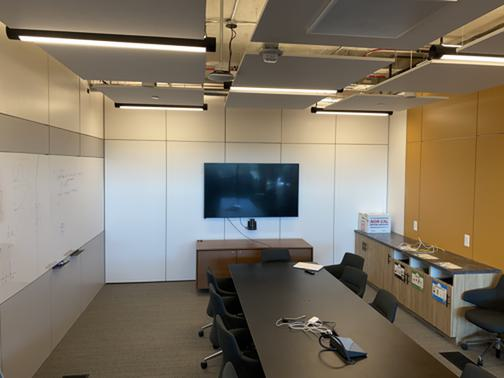
\includegraphics[width=.96\linewidth]{figures/llff/room_gt.jpg}
    \caption{Ground Truth}
    \label{fig:llff_gt}
\end{subfigure}%
\begin{subfigure}{.25\textwidth}
    \centering
    \captionsetup{justification=centering}
    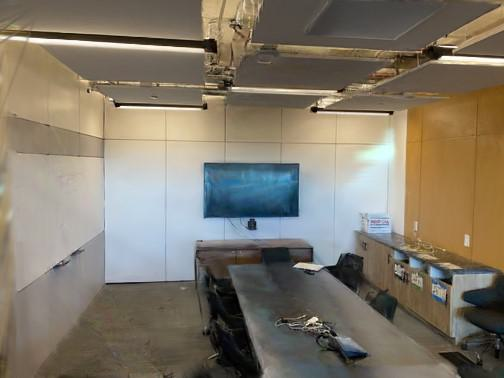
\includegraphics[width=.96\linewidth]{figures/llff/room_interngs.jpg}
    \caption{Intern-GS}
    \label{fig:llff_interngs}
\end{subfigure}
\vspace{0.3cm}
\begin{subfigure}{.25\textwidth}
    \centering
    \captionsetup{justification=centering}
    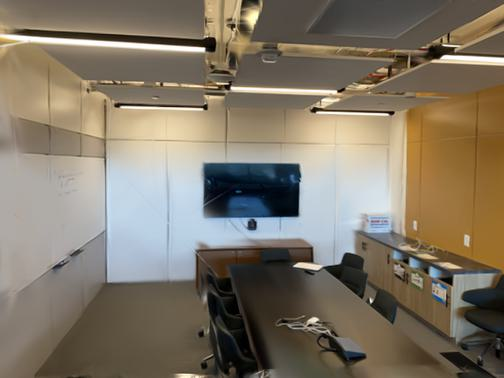
\includegraphics[width=.96\linewidth]{figures/llff/room_ours.jpg}
    \caption{Ours}
    \label{fig:llff_ours}
\end{subfigure}
\caption{The Figures show a comparison between Intern-GS~\cite{InternGS}, Ours and the Ground Truth. Our model has very accurate reflections and fewer artifacts, nevertheless our model can not correctly reconstruct the unseen region at the ceiling.}
\label{fig:llff_example}
\end{figure}

\cref{tab:evaluation_mipnerf360_3view} shows the comparison between Gaussian Scenes, MASt3R Initialization, FSGS and Our method in the 3-view setting on MipNeRF360~\cite{GaussianScenes, fsgs}. Our model achieves the lowest LPIPS score and second highest PSNR and SSIM. Compared to FSGS our model does not rely on accurate camera poses from traditional SfM.

\cref{tab:evaluation_mipnerf360_12view} shows the comparison between 3DGS, \textit{DNGaussian}, \textit{SparseGS} and Our method in 12-view setting on MipNeRF360~\cite{mipnerf360}. Our model achieves the highest results with very coherent and view-consistent final scene, as our model improves the Gaussian surface alignment significantly. A comparison can be seen in \cref{fig:garden_example}.\\
To validate the accuracy of our camera pose estimates, we evaluate the Absolute Trajectory Error (ATE) on the Tank and Temples dataset. Our pose estimator, $\pi^3$, achieves a mean ATE of 0.0293 and a root mean squared error (RMSE) of 0.0325, demonstrating that it produces accurate camera poses suitable for fair comparison of photometric metrics in 3D Gaussian splatting.

\begin{figure}
\centering
\begin{subfigure}{.25\textwidth}
    \centering
    \captionsetup{justification=centering}
    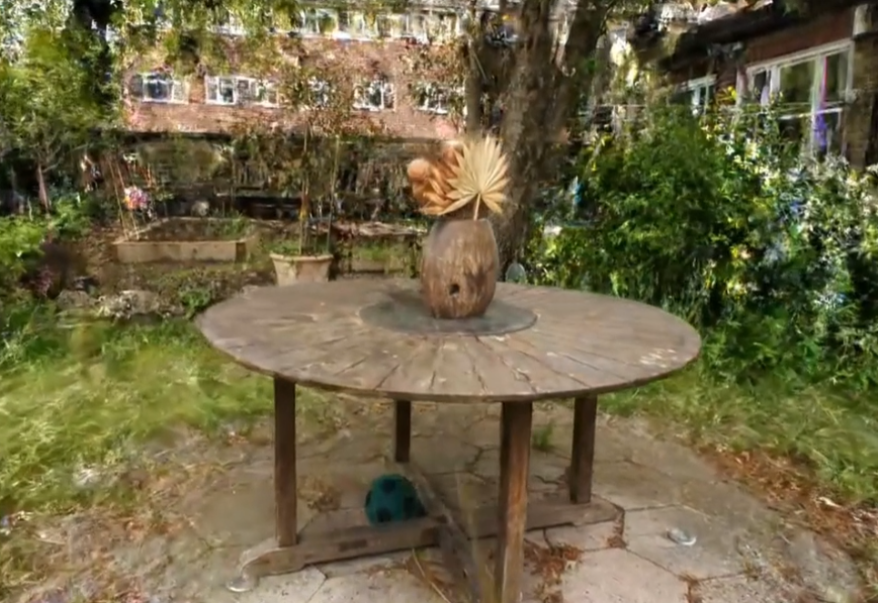
\includegraphics[width=.96\linewidth]{figures/garden_sparsegs.png}
    \caption{SparseGS}
    \label{fig:garden_sparsegs}
\end{subfigure}%
\begin{subfigure}{.25\textwidth}
    \centering
    \captionsetup{justification=centering}
    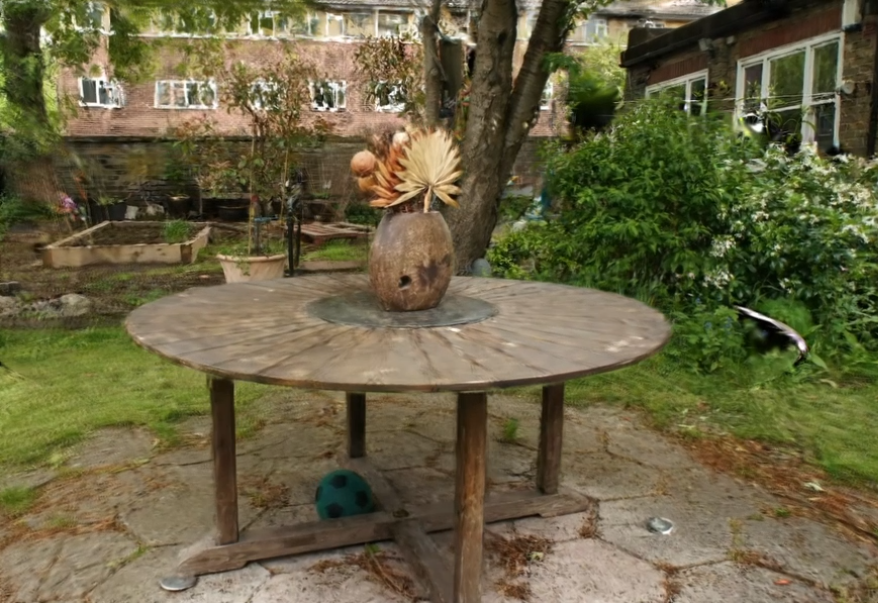
\includegraphics[width=.96\linewidth]{figures/garden_ours.png}
    \caption{Ours}
    \label{fig:garden_ours}
\end{subfigure}
\caption{The Figures show a comparison between SparseGS~\cite{SparseGS} and our method. Our model reconstructs the background and ground more accurately, and additionally decreases artifacts.}
\label{fig:garden_example}
\end{figure}

\subsection{Ablation}
We evaluate the impact of each individual optimization on our final result.
The evaluation is conducted using the Barn scene from the Tanks and Temples dataset. It is evident that all of our optimizations improve the result even further. Dense point cloud initialization with the help of $\pi^3$ significantly improves the result by also reducing the time required for SfM.
Our custom depth loss improves the score by allowing low confidence depth regions to optimize more freely.
Normal regularization encourages the Gaussians' normals to match the ground-truth geometry. Depth warping improves the results by adding more views, which helps the model generalize better and avoid overfitting to the training views.
Our full model achieves a PSNR of \textit{22.15} on the Barn scene. We also evaluated the effect of enabling splitting of Gaussians in our model. This setting results in a slight decrease in performance and was therefore deactivated. These results can be seen in \cref{tab:ablation}.
\begin{table}[ht!]
    \centering
    \footnotesize
    \setlength{\tabcolsep}{2pt}
    \begin{tabular}{lc}
    \toprule
     Method & PSNR\\
     \midrule
 Original 3DGS & 17.53\\
 PGSR & 18.05\\
 $\pi^3$ (dense) initialization & 19.66\\
 + Depth Regularization & 20.72\\
 + Normal Regularization & \cellcolor{tab_color!10}21.56\\
 + Depth Warping (Full Model) & \cellcolor{tab_color!50}{22.15}\\
 \midrule
 + Splitting Densification &\cellcolor{tab_color!30}21.97\\
    \bottomrule
    \end{tabular}
    \caption{Ablation study of the regularization techniques introduced in our model on the Barn scene of Tanks and Temples. Additionally, we evaluated the impact of splitting Gaussians during densification.}
    \label{tab:ablation}
\end{table}

In addition, we evaluate the impact of using PGSR compared to standard 3DGS for our sparse view setting (3-views).
\Cref{tab:evaluation_3dgs_pgsr} shows that the planar depth created by PGSR helps significantly to place the Gaussians more accurately. Additionally, the losses introduced by PGSR help to improve the rendering results further. Our model remains stable even after increased training iterations and continues to show improved novel view synthesis results.
A visual comparison between 3DGS and PGSR with different number of iterations can be seen in \cref{fig:pgsr_vs_3dgs}.
\begin{table}[ht!]
    \centering
    \footnotesize
    \setlength{\tabcolsep}{2pt}
    \resizebox{\columnwidth}{!}{\begin{tabular}{lccccccc}
    \toprule
    \multirow{3}{*}{Framework} & \multirow{3}{*}{Iteration} &\multicolumn{3}{c}{Tanks and Temples} & \multicolumn{3}{c}{MipNeRF360}\\
    \cmidrule(lr){3-5} \cmidrule(lr){6-8}
    && PSNR\textsuperscript{$\uparrow$} & SSIM\textsuperscript{$\uparrow$} & LPIPS\textsuperscript{$\downarrow$}& PSNR\textsuperscript{$\uparrow$} & SSIM\textsuperscript{$\uparrow$} & LPIPS\textsuperscript{$\downarrow$}\\
    \midrule
    PGSR~\cite{pgsr2024} & 7000  & \cellcolor{tab_color!30}19.99 & \cellcolor{tab_color!30}0.503 & \cellcolor{tab_color!30}0.355 & \cellcolor{tab_color!30}23.36 & \cellcolor{tab_color!30}0.791 & \cellcolor{tab_color!50}0.156\\
    3DGS~\cite{3dgs2023} & 7000  & \cellcolor{tab_color!10}18.00 & \cellcolor{tab_color!10}0.426 & \cellcolor{tab_color!10}0.449 & \cellcolor{tab_color!10}23.07 & \cellcolor{tab_color!10}0.773 & \cellcolor{tab_color!10}0.172\\
    \midrule
    PGSR~\cite{pgsr2024} & 15000 & \cellcolor{tab_color!50}20.19 & \cellcolor{tab_color!50}0.517 & \cellcolor{tab_color!50}0.343 & \cellcolor{tab_color!50}23.41 & \cellcolor{tab_color!50}0.795 & \cellcolor{tab_color!30}0.169\\
    3DGS~\cite{3dgs2023} & 15000 & 17.04 & 0.391 & 0.465 & 20.94 & 0.719 & 0.244\\
    \bottomrule
    \end{tabular}}
    \caption{Ablation study on the use of PGSR as base framework compared to 3DGS. The additional multi-view and single-view losses introduced by PGSR are activated after iteration 7000. This comparison shows that the PGSR depth rendering captures the underlying surface geometry more accurately by also reducing floaters significantly. With the help of PGSR we achieve view-consistent surfaces and reduce overfitting significantly.}
    \label{tab:evaluation_3dgs_pgsr}
\end{table}
\begin{figure*}[t]
\centering
\setlength{\tabcolsep}{.5pt}
\small
\begin{tabular}{r @{\hspace{0.3cm}} c c c c}
    \multicolumn{1}{l}{\textbf{Scene}} &
    \multicolumn{2}{c}{\textbf{3DGS~\cite{3dgs2023}}} &
    \multicolumn{2}{c}{\textbf{PGSR~\cite{pgsr2024}}}\\
    \multicolumn{1}{c}{\textbf{}} &
    \multicolumn{1}{c}{\textbf{7K Iterations}} &
    \multicolumn{1}{c}{\textbf{15K Iterations}} &
    \multicolumn{1}{c}{\textbf{7K Iterations}} &
    \multicolumn{1}{c}{\textbf{15K Iterations}}\\[0.2cm]\vspace{-0.25em}
    %
    \raisebox{4.0\height}{\textbf{Barn~\cite{tankstemples}}} &
    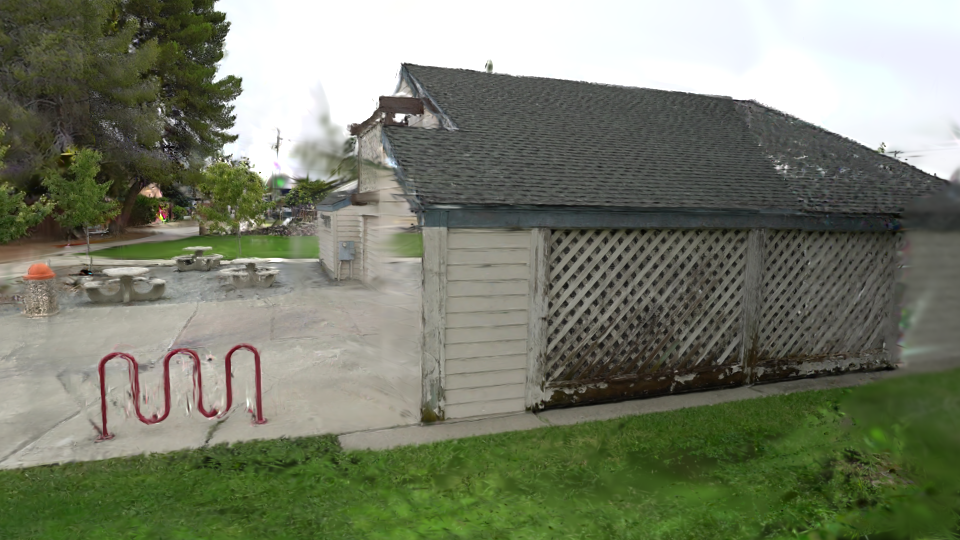
\includegraphics[width=.19\linewidth]{figures/PGSR_vs_3DGS/3DGS_barn_7000.png} &
    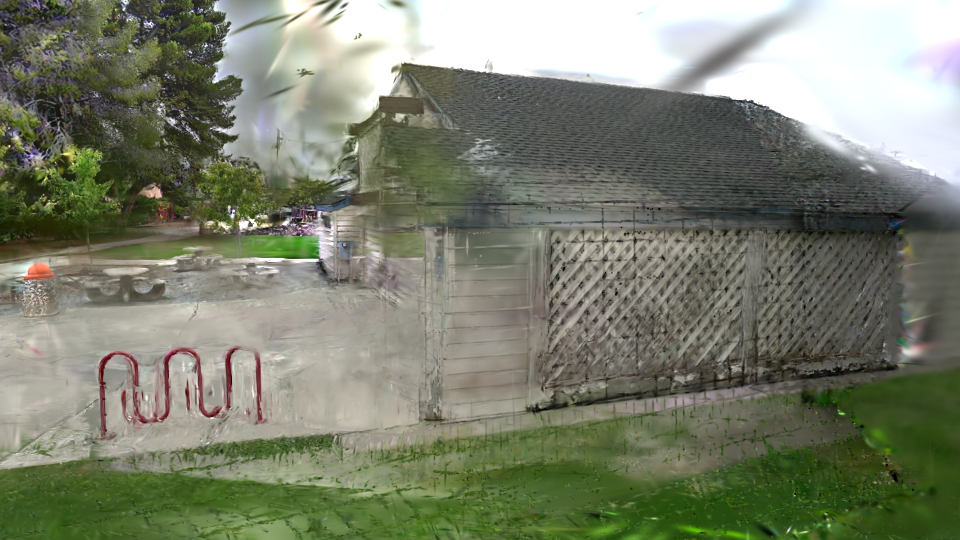
\includegraphics[width=.19\linewidth]{figures/PGSR_vs_3DGS/3DGS_barn_15000.png} &
    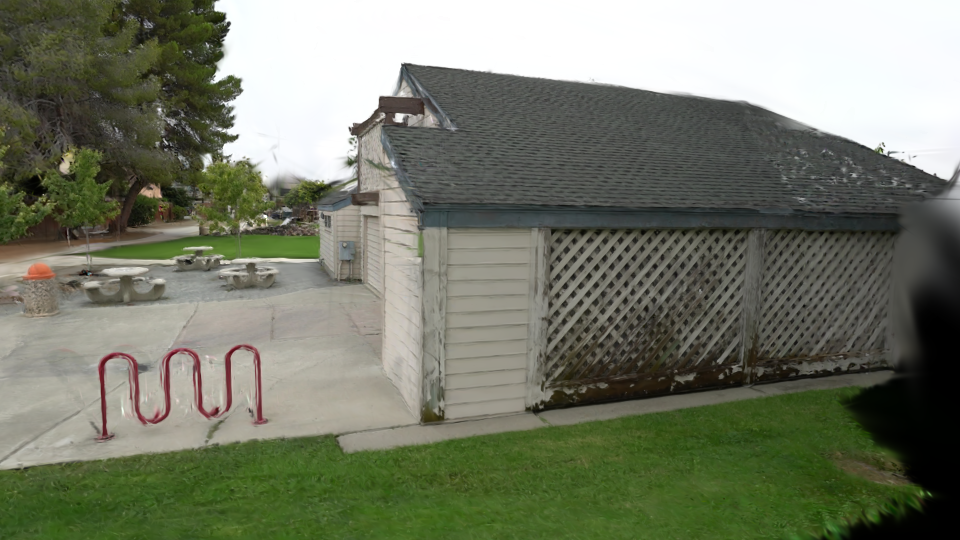
\includegraphics[width=.19\linewidth]{figures/PGSR_vs_3DGS/PGSR_barn_7000.png} &
    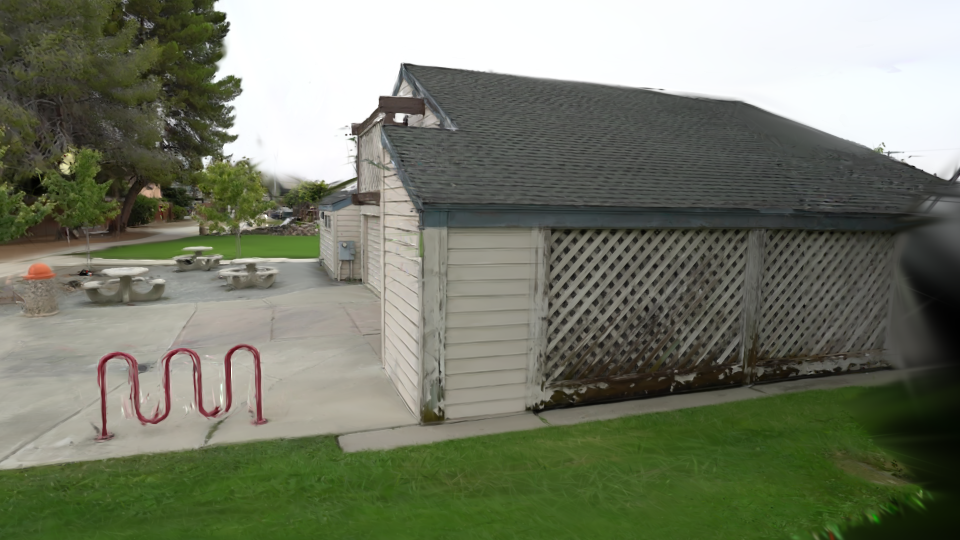
\includegraphics[width=.19\linewidth]{figures/PGSR_vs_3DGS/PGSR_barn_15000.png}\\\vspace{-0.25em}
    %
    \raisebox{4.0\height}{\textbf{Ballroom~\cite{tankstemples}}} &
    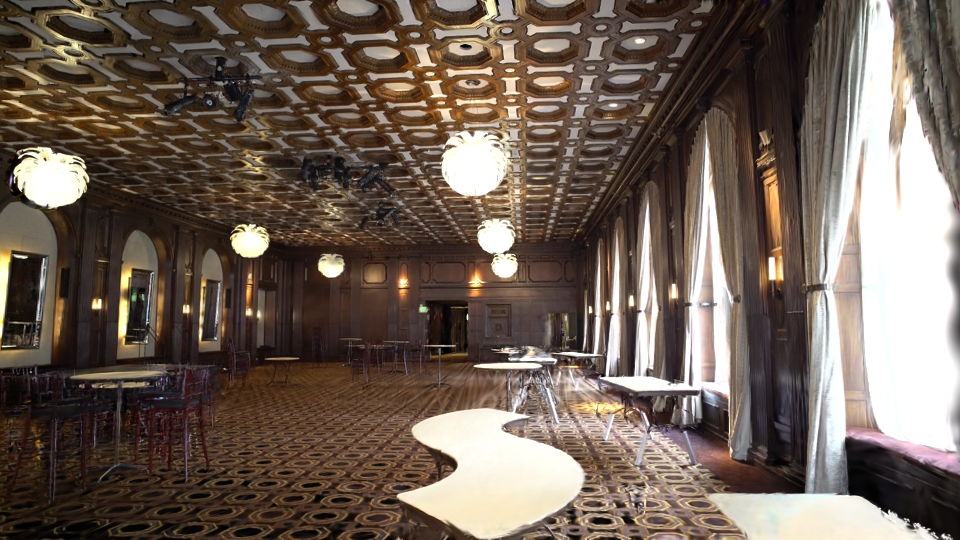
\includegraphics[width=.19\linewidth]{figures/PGSR_vs_3DGS/3DGS_ballroom_7000.png} &
    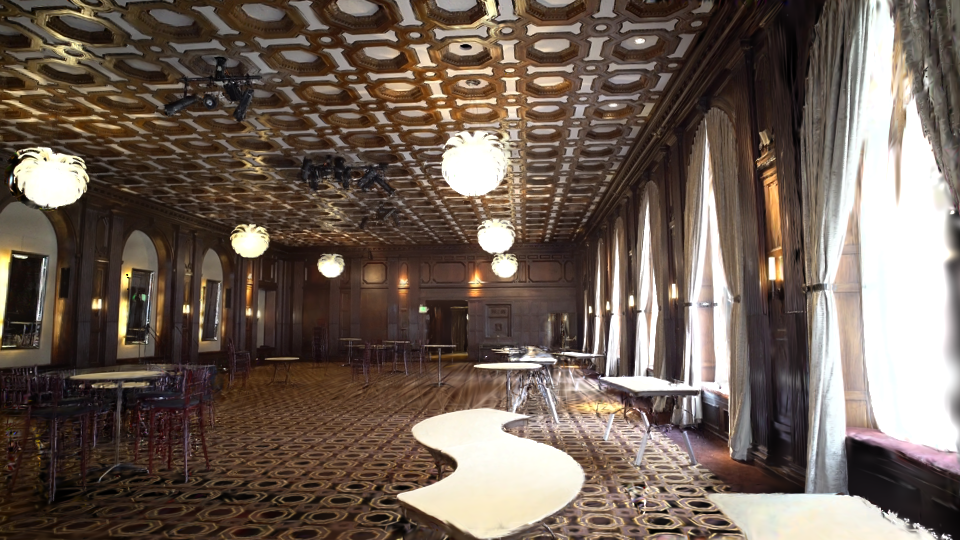
\includegraphics[width=.19\linewidth]{figures/PGSR_vs_3DGS/3DGS_ballroom_15000.png} &
    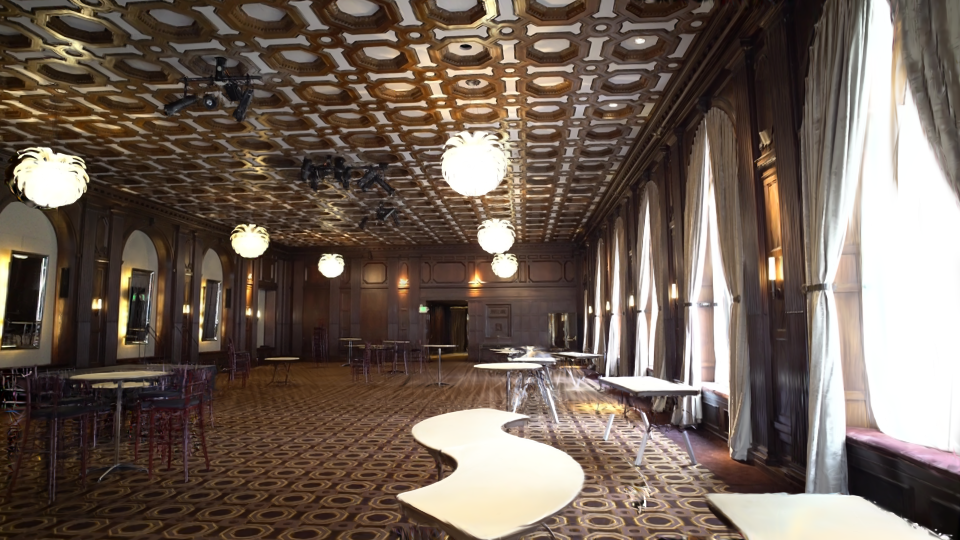
\includegraphics[width=.19\linewidth]{figures/PGSR_vs_3DGS/PGSR_ballroom_7000.png} &
    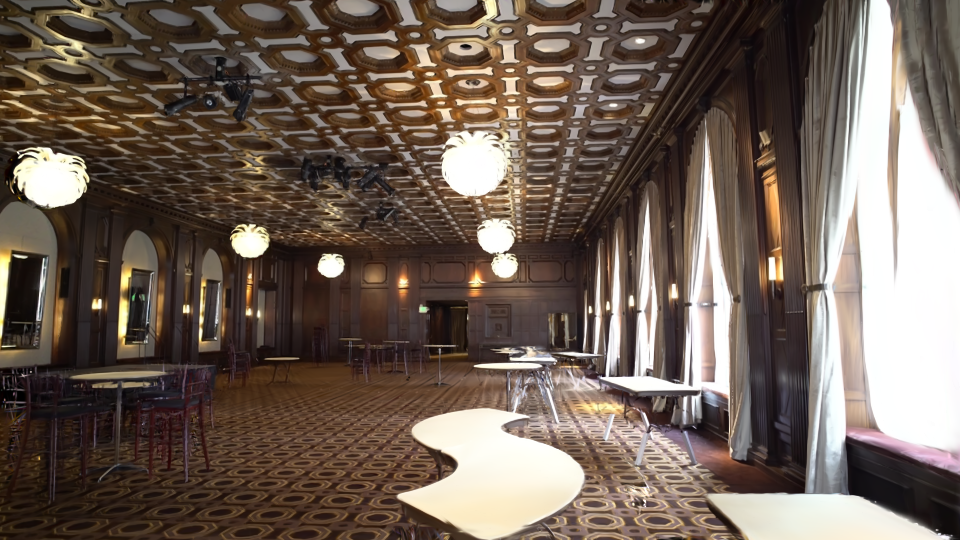
\includegraphics[width=.19\linewidth]{figures/PGSR_vs_3DGS/PGSR_ballroom_15000.png}\\\vspace{-0.25em}
    %
    \raisebox{4.0\height}{\textbf{Kitchen~\cite{mipnerf360}}} &
    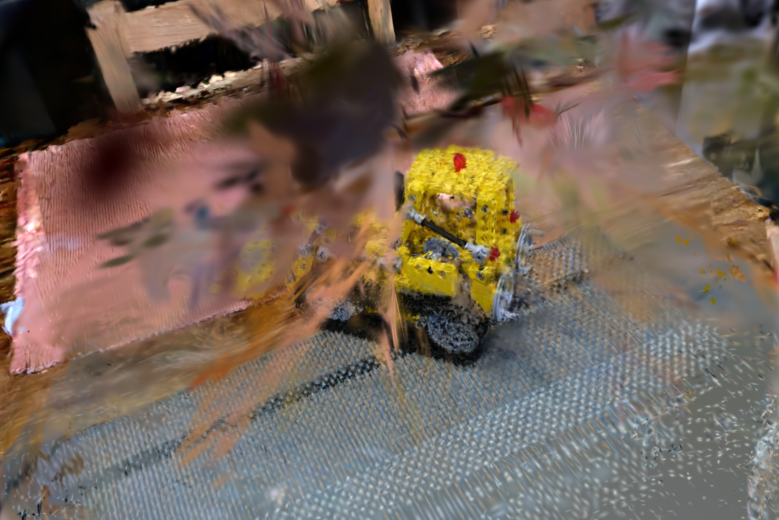
\includegraphics[width=.19\linewidth]{figures/PGSR_vs_3DGS/3DGS_kitchen_7000.png} &
    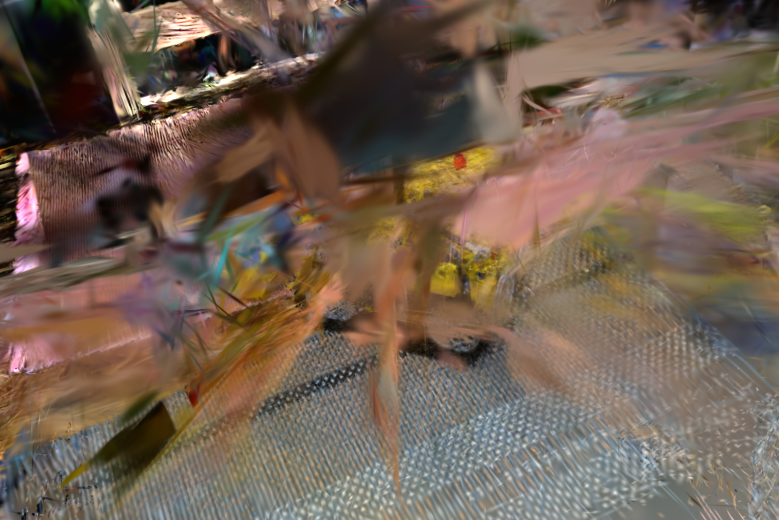
\includegraphics[width=.19\linewidth]{figures/PGSR_vs_3DGS/3DGS_kitchen_15000.png} &
    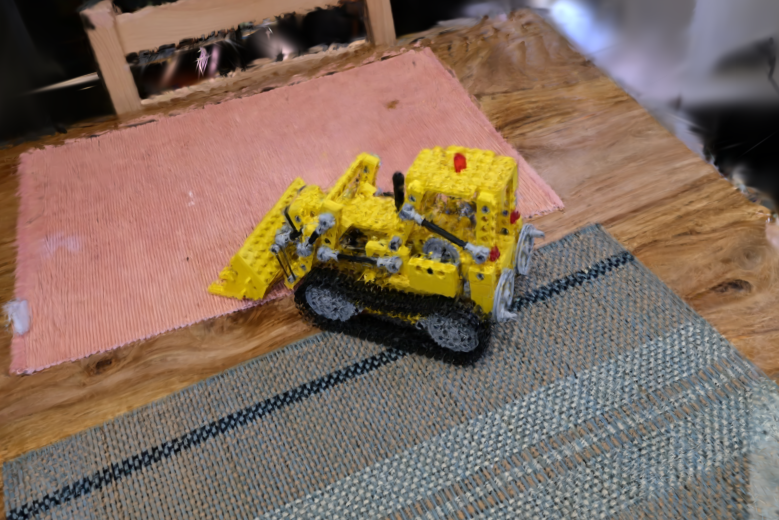
\includegraphics[width=.19\linewidth]{figures/PGSR_vs_3DGS/PGSR_kitchen_7000.png} &
    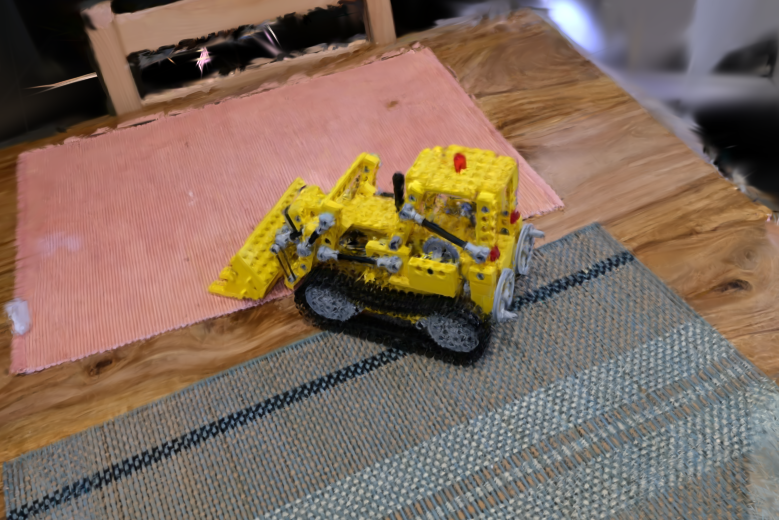
\includegraphics[width=.19\linewidth]{figures/PGSR_vs_3DGS/PGSR_kitchen_15000.png}\\\vspace{-0.25em}
    %
    \raisebox{4.0\height}{\textbf{Garden~\cite{mipnerf360}}} &
    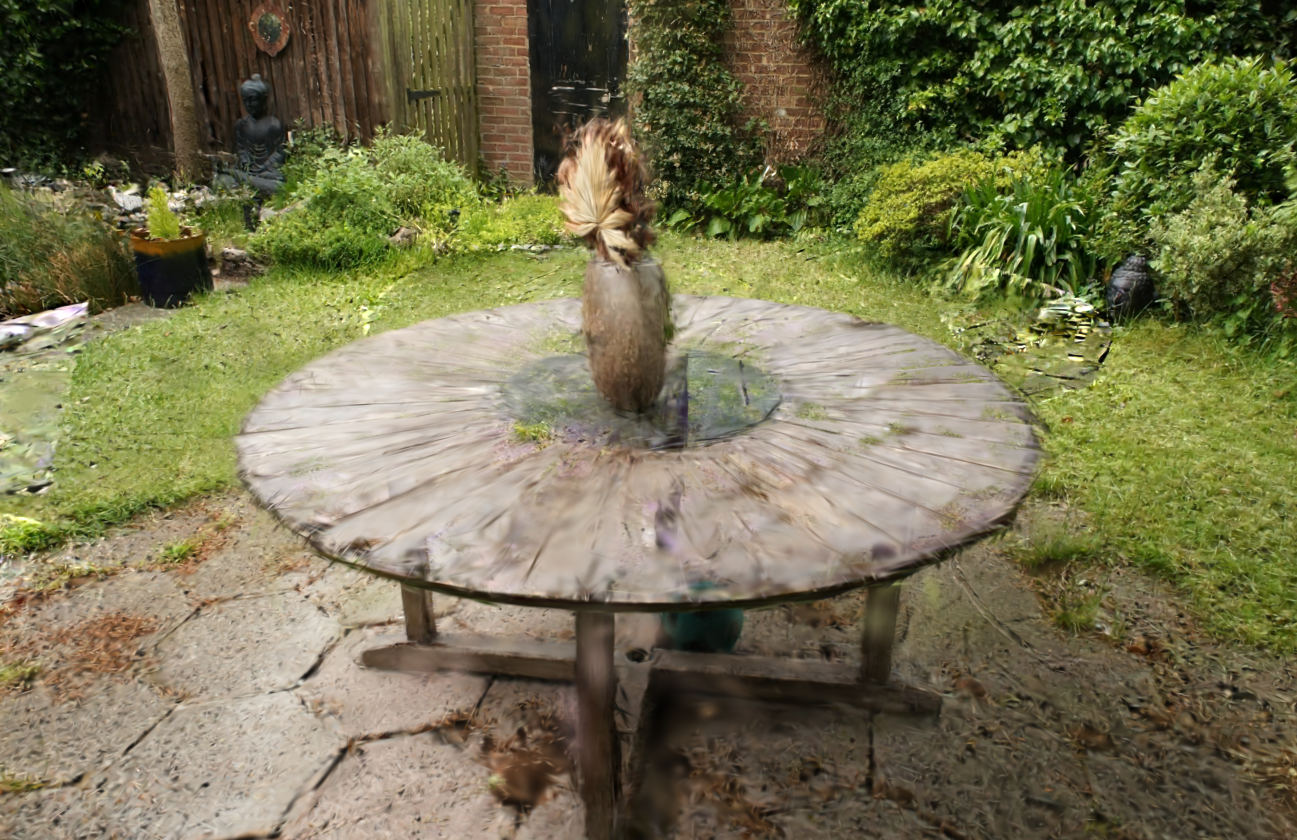
\includegraphics[width=.19\linewidth]{figures/PGSR_vs_3DGS/3DGS_garden_7000.png} &
    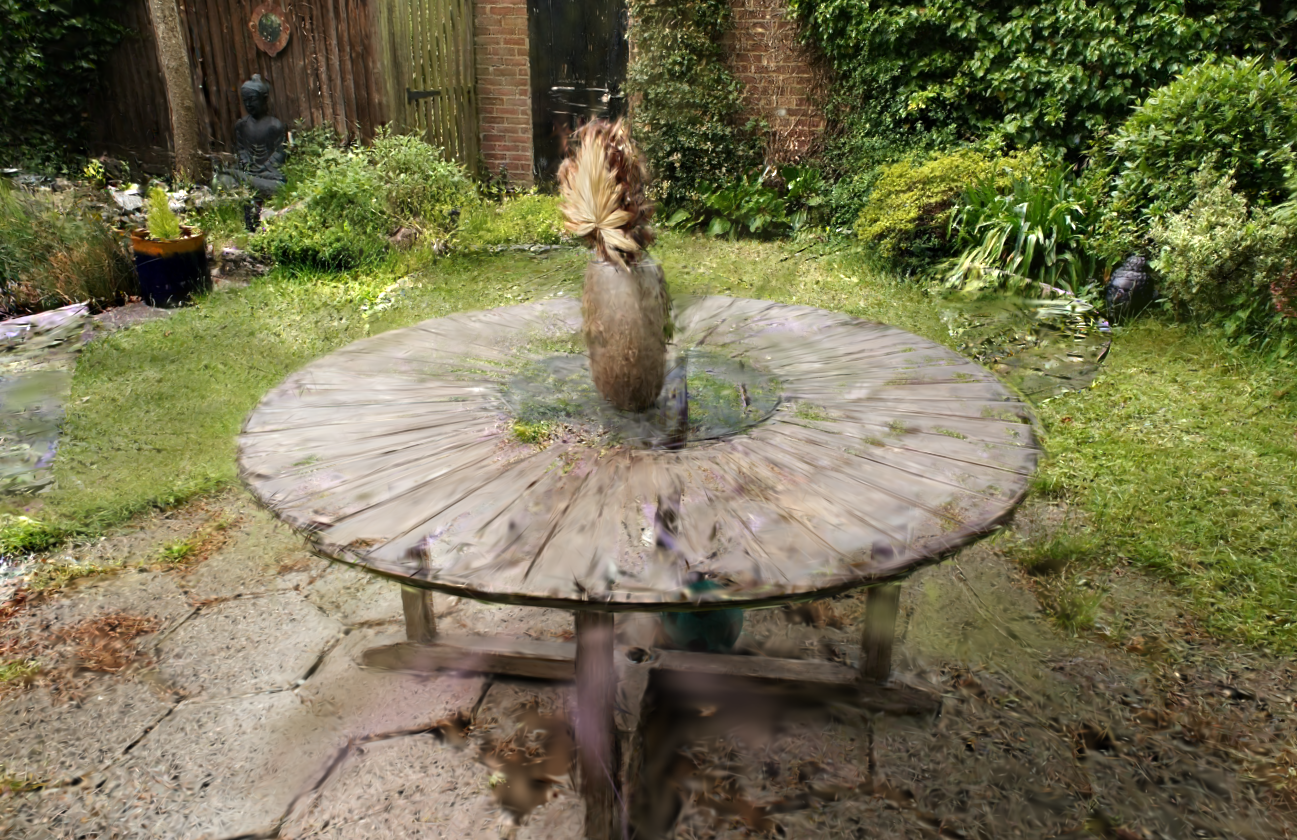
\includegraphics[width=.19\linewidth]{figures/PGSR_vs_3DGS/3DGS_garden_15000.png} &
    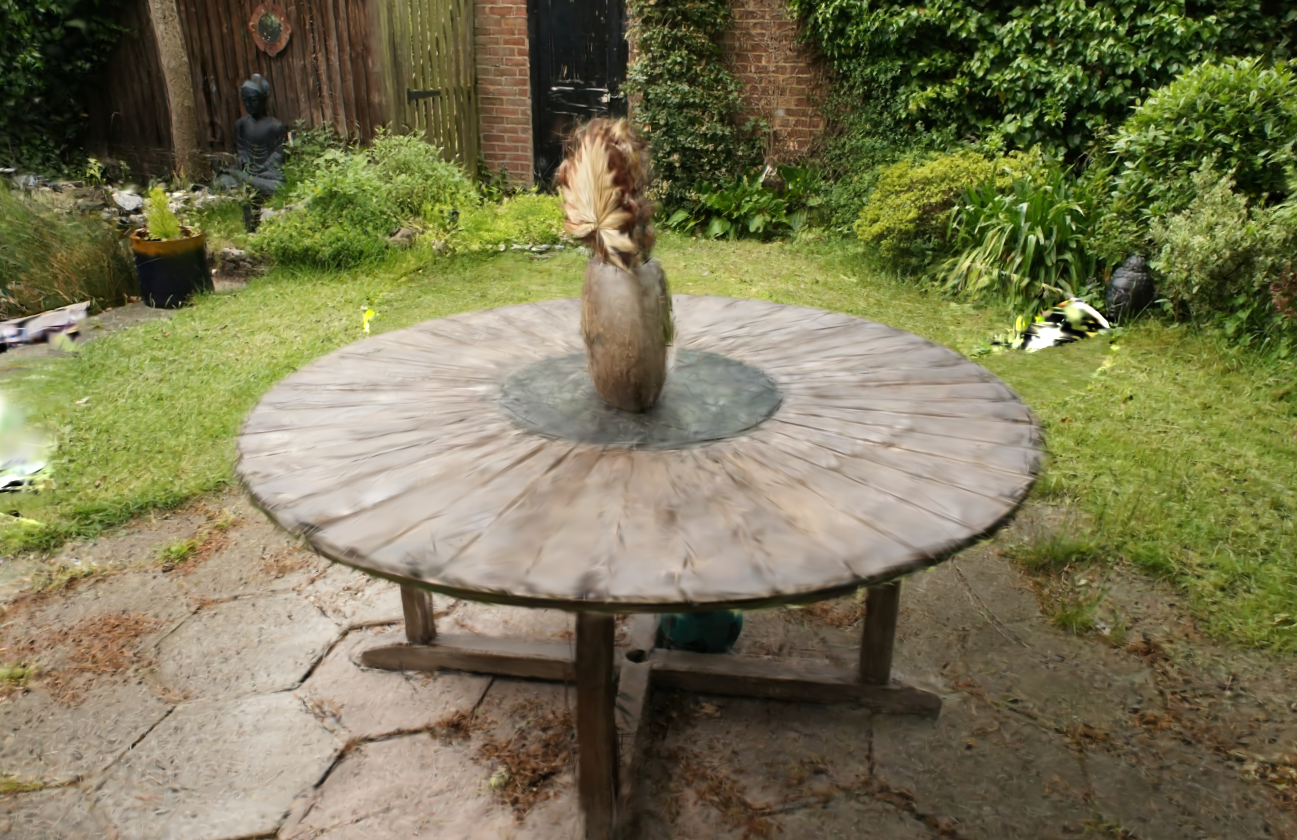
\includegraphics[width=.19\linewidth]{figures/PGSR_vs_3DGS/PGSR_garden_7000.png} &
    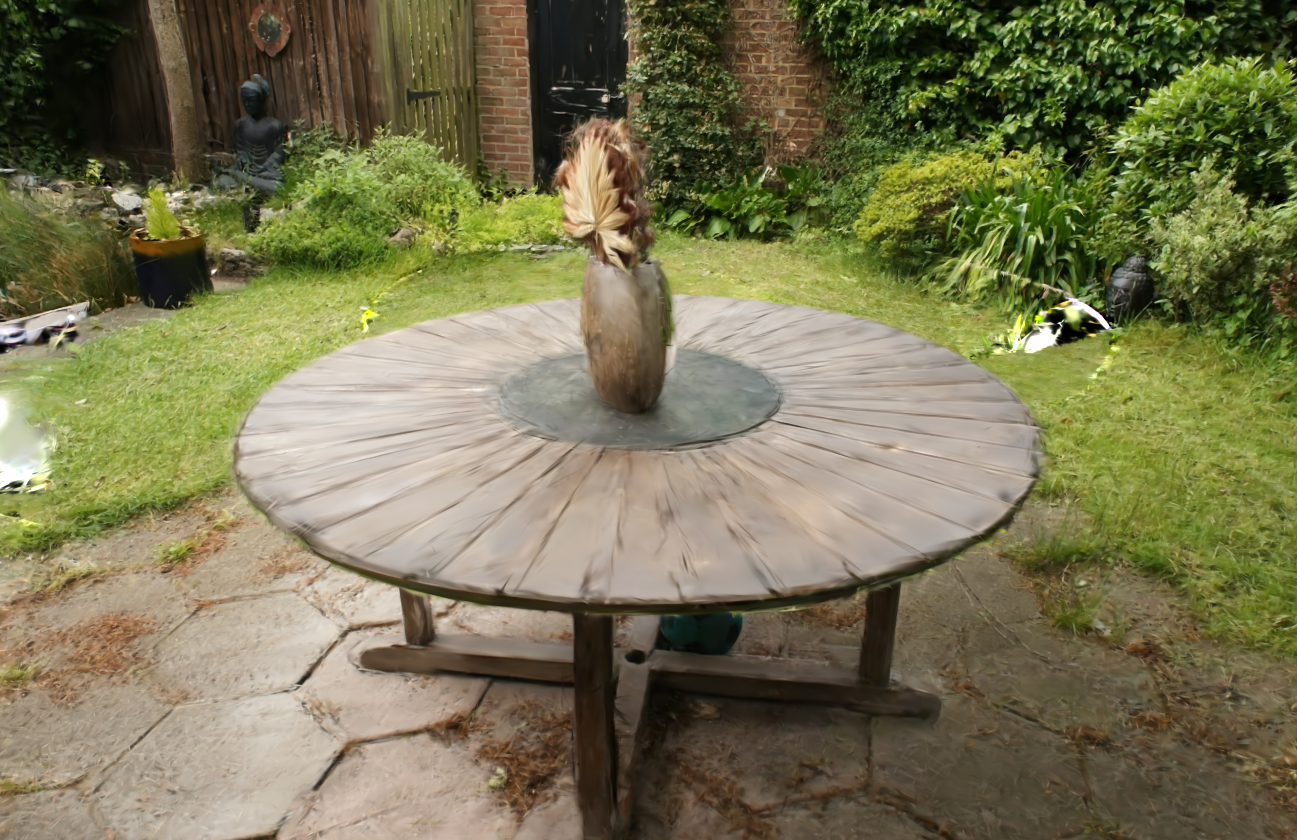
\includegraphics[width=.19\linewidth]{figures/PGSR_vs_3DGS/PGSR_garden_15000.png}\\\vspace{-0.25em}
\end{tabular}
\vspace{-0.2cm}
\caption{Visual comparison between 3DGS and PGSR with different Iterations. The planar depth from PGSR helps significantly to remove floaters and align the Gaussians accurately to the ground-truth geometry.}
\label{fig:pgsr_vs_3dgs}
\end{figure*}

\begin{table}[ht!]
    \centering
    \footnotesize
    \setlength{\tabcolsep}{2pt}
    \begin{tabular}{lccc}
    \toprule
     Method & PSNR\textsuperscript{$\uparrow$} & SSIM\textsuperscript{$\uparrow$} & LPIPS\textsuperscript{$\downarrow$}\\
    \midrule
 3DGS~\cite{3dgs2023} & 15.36 & 0.572 & 0.379 \\
 DNGaussian~\cite{DNGaussian} & 20.69 & 0.721 & 0.277 \\
 SparseGS~\cite{SparseGS} & 21.20 & 0.717 & 0.231 \\
 InstantSplat~\cite{InstantSplat} & 22.20 & \cellcolor{tab_color!30}{0.743} & 0.199 \\
 FSGS~\cite{fsgs}&\cellcolor{tab_color!10}22.31& 0.693&\cellcolor{tab_color!10}0.197\\
 Intern-GS~\cite{InternGS} & \cellcolor{tab_color!30}{22.67} & \cellcolor{tab_color!10}0.736 & \cellcolor{tab_color!30}{0.191} \\
 Ours & \cellcolor{tab_color!50}{22.87} & \cellcolor{tab_color!50}{0.764} & \cellcolor{tab_color!50}{0.189}\\
    \bottomrule
    \end{tabular}
    \caption{Evaluation on Tanks and Temples dataset with 3-view setting. Our model does not oversmooth high-frequency textures and accurately aligns the Gaussians with the underlying surface geometry.}
    \label{tab:evaluation_tat}
\end{table}
\begin{table}[ht!]
    \centering
    \footnotesize
    \setlength{\tabcolsep}{2pt}
    \begin{tabular}{lccc}
    \toprule
    Method & PSNR\textsuperscript{$\uparrow$} & SSIM\textsuperscript{$\uparrow$} & LPIPS\textsuperscript{$\downarrow$}\\
    \midrule
 MASt3R Initialization~\cite{GaussianScenes} & 12.59 & 0.231 & 0.593 \\ 
 Gaussian Scenes~\cite{GaussianScenes} & \cellcolor{tab_color!10}{13.81} & \cellcolor{tab_color!10}{0.265} & \cellcolor{tab_color!30}{0.547} \\ 
 FSGS~\cite{fsgs} & \cellcolor{tab_color!50}14.17 & \cellcolor{tab_color!50}0.318 & \cellcolor{tab_color!10}0.578 \\
 %GenFusion~\cite{GenFusion} & 15.29 & 0.369 & 0.585 \\
 Ours & \cellcolor{tab_color!30}14.14 & \cellcolor{tab_color!30}{0.310} & \cellcolor{tab_color!50}{0.523}\\
    \bottomrule
    \end{tabular}
    \caption{Evaluation on MipNeRF360 dataset with 3-view setting. Our model reconstructs seen regions accurately, but can not introduce geometry in unseen regions.}
    \label{tab:evaluation_mipnerf360_3view}
\end{table}
\begin{table}[ht!]
    \centering
    \footnotesize
    \setlength{\tabcolsep}{2pt}
    \begin{tabular}{lccc}
    \toprule
     Method & PSNR\textsuperscript{$\uparrow$} & SSIM\textsuperscript{$\uparrow$} & LPIPS\textsuperscript{$\downarrow$}\\
     \midrule
 3DGS~\cite{3dgs2023} & \cellcolor{tab_color!10}17.49 & \cellcolor{tab_color!10}0.490 & \cellcolor{tab_color!10}0.431 \\
 DNGaussian~\cite{DNGaussian} & 16.28 & 0.432 & 0.549 \\
 SparseGS~\cite{SparseGS} & \cellcolor{tab_color!30}{19.37} & \cellcolor{tab_color!50}{0.577} & \cellcolor{tab_color!30}{0.398} \\
 Ours & \cellcolor{tab_color!50}{19.54} & \cellcolor{tab_color!30}{0.492} & \cellcolor{tab_color!50}{0.362}\\
    \bottomrule
    \end{tabular}
    \caption{Evaluation on MipNeRF360 dataset with 12-view setting. Our model can reconstruct the scenes with highly accurate surface alignment. The ground is view-consistent, and fewer floating artifacts compared to SparseGS~\cite{SparseGS}.}
    \label{tab:evaluation_mipnerf360_12view}
\end{table}
\begin{table}[ht!]
    \centering
    \footnotesize
    \setlength{\tabcolsep}{2pt}
    \begin{tabular}{lcccccc}
    \toprule
    \multirow{3}{*}{Method} & \multicolumn{3}{c}{LLFF} & \multicolumn{3}{c}{DTU}\\
    \cmidrule(lr){2-4} \cmidrule(lr){5-7}
    & PSNR\textsuperscript{$\uparrow$} & SSIM\textsuperscript{$\uparrow$} & LPIPS\textsuperscript{$\downarrow$}& PSNR\textsuperscript{$\uparrow$} & SSIM\textsuperscript{$\uparrow$} & LPIPS\textsuperscript{$\downarrow$}\\
    \midrule
 3DGS~\cite{3dgs2023} & 15.52 & 0.408 & 0.405&10.99 & 0.585 & 0.313 \\ 
 DNGaussian~\cite{DNGaussian} & 19.12 & 0.591 & \cellcolor{tab_color!10}0.294&\cellcolor{tab_color!10}18.91 & 0.790 & \cellcolor{tab_color!10}0.176 \\ 
 SparseGS~\cite{SparseGS} & 19.86 & \cellcolor{tab_color!30}{0.668} & 0.322& 18.89 & \cellcolor{tab_color!30}0.834 & 0.178 \\ 
 InstantSplat~\cite{InstantSplat} & 17.67 & 0.603 & 0.379&17.55 & 0.634 & 0.212 \\ 
 FSGS~\cite{fsgs}&\cellcolor{tab_color!30}20.31& 0.652&0.288&19.54& 0.732&0.199\\
 Intern-GS~\cite{InternGS} & \cellcolor{tab_color!50}{20.49} &  \cellcolor{tab_color!50}{0.693} & \cellcolor{tab_color!50}{0.212}&\cellcolor{tab_color!30}{20.34} & \cellcolor{tab_color!50}{0.851} & \cellcolor{tab_color!30}{0.163} \\ 
 Ours & \cellcolor{tab_color!10}19.92 & \cellcolor{tab_color!10}0.664 & \cellcolor{tab_color!30}{0.254}&\cellcolor{tab_color!50}{23.52} & \cellcolor{tab_color!10}{0.815} & \cellcolor{tab_color!50}{0.145}\\
    \bottomrule
    \end{tabular}
    \caption{Evaluation on LLFF and DTU dataset with 3-view setting. Following previous work, for evaluation on DTU the background masks are applied. Our model is able to reconstruct fine-grained textures accurately, but it underperforms in unobserved regions compared to methods that generate content for unseen regions.}
    \label{tab:llff_dtu_comparison}
\end{table}

%\input{tables/LLFF_comparison}
%\input{tables/DTU_comparison}
